\chapter{PEFT for Post-Training}
\label{ch:peft}
\raggedbottom

In 2023, QLoRA made a surprising claim: a 65B-parameter language model could be fine-tuned on a single 48\,GB GPU~\cite{dettmers2023qlora}. A year earlier, this sounded like a cluster job. The loss function had not changed. The instruction data had not magically become smaller. What changed was the memory layout: freeze the pretrained model, train a tiny low-rank update, and store the frozen base in 4-bit precision.

That result matters because Chapter~\ref{ch:instruction-tuning} taught you a recipe that is conceptually simple but hardware-hostile: take a pretrained model, choose instruction data, compute masked cross-entropy, and train for a few epochs. The mathematical recipe fits in one line. The optimizer state does not.

A 7-billion-parameter model stored in 16-bit precision occupies 14\,GB of GPU memory---just for the weights. Add gradients (14\,GB), Adam optimizer states (56\,GB for first and second moments in 32-bit), and master weights (28\,GB in 32-bit), and you need roughly 112\,GB of GPU memory before a single activation tensor is allocated. A consumer-grade GPU has 24\,GB. The recipe from Chapter~\ref{ch:instruction-tuning} is correct but, at the parameter counts that matter, it does not fit.

This chapter solves that problem. It introduces \emph{parameter-efficient fine-tuning} (PEFT): methods that update only a small fraction of the model's parameters, reducing peak memory by $4$--$16\times$ and making fine-tuning possible on a single consumer GPU. The most important of these methods is LoRA (Low-Rank Adaptation), and most of this chapter is about LoRA and its quantized variant, QLoRA.

But PEFT is not just an engineering trick. It works because of a deep empirical fact: fine-tuning does not need most of the parameter space. The update often lives in a low-dimensional subspace far smaller than the full weight matrix. Chapter~\ref{ch:instruction-tuning} argued \emph{behaviorally} that SFT surfaces existing capability rather than teaching new knowledge. This chapter makes the \emph{mathematical} version of the same claim: fine-tuning usually redirects a pretrained model through a small update, not a wholesale rewrite. LoRA is the engineering consequence of that fact.

\paragraph{What this chapter covers.} Three ideas organize the chapter. First, full fine-tuning runs into a memory wall that is different from the pretraining memory wall (\S\ref{sec:memory-wall-peft}). Second, LoRA and QLoRA make the update small enough to fit on accessible hardware (\S\ref{sec:lora-math}--\S\ref{sec:qlora}). Third, PEFT becomes a decision framework for the rest of Part~III: when to use full fine-tuning, when to use LoRA, when to use QLoRA, and why preference learning and RL methods depend on the same infrastructure (\S\ref{sec:other-peft}--\S\ref{sec:peft-pipeline}).

\paragraph{Running example.} Project~3 asks you to instruction-tune a 3B model on a single 24\,GB GPU. Section by section, this chapter will show why full fine-tuning does not fit, how LoRA makes it tight, and how QLoRA makes it comfortable.

\subsection*{Learning Objectives}

After completing this chapter, you should be able to:

\begin{enumerate}
  \item Compute the peak GPU memory required for full fine-tuning of a given model size and explain why this exceeds a single-GPU budget at 3B+ parameters.
  \item Write the LoRA forward pass $h = (W + \frac{\alpha}{r} BA)x$ and explain the role of each component.
  \item Explain the $\alpha/r$ scaling factor and why changing rank without adjusting $\alpha$ changes the effective learning rate.
  \item Describe the intrinsic dimensionality hypothesis and connect it to the LIMA ``surfacing'' thesis from Chapter~\ref{ch:instruction-tuning}.
  \item Explain NF4 quantization and why it outperforms uniform INT4 for neural network weights.
  \item Given a model size, available GPU memory, and task type, select the appropriate fine-tuning strategy (full FT, LoRA, or QLoRA).
  \item Explain why PEFT is essential for DPO, RLHF, and reasoning RL, and describe how LoRA changes the memory layout for DPO.
\end{enumerate}


\subsection*{Notation}

\begin{center}
\begin{tabular}{ll}
\toprule
Symbol & Meaning \\
\midrule
$W$ & Frozen pretrained weight matrix ($d \times d$ or $d_{\text{out}} \times d_{\text{in}}$) \\
$B, A$ & LoRA low-rank matrices: $B \in \mathbb{R}^{d \times r}$, $A \in \mathbb{R}^{r \times d}$ \\
$r$ & LoRA rank (typically 8--64) \\
$\alpha$ & LoRA scaling factor \\
$\Delta W$ & Weight update: $\Delta W = \frac{\alpha}{r} B A$ \\
$d$ & Hidden dimension of the model \\
$\theta$ & Model parameters \\
\bottomrule
\end{tabular}
\end{center}


\subsection*{Timeline}

\begin{center}
\begin{tabularx}{\textwidth}{@{}lX@{}}
\toprule
\textbf{Year} & \textbf{Milestone} \\
\midrule
2019 & Houlsby et al.: adapter layers inserted between Transformer blocks \\
2021 & Li \& Liang: prefix tuning---learnable tokens prepended to keys and values \\
2021 & Aghajanyan et al.: fine-tuning has low intrinsic dimensionality (the conceptual foundation for LoRA) \\
2021 & Hu et al. (LoRA): low-rank adaptation of large language models \\
2023 & Dettmers et al. (QLoRA): 4-bit quantization plus LoRA; 65B model fine-tuned on a single 48\,GB GPU \\
2024 & Liu et al. (DoRA): weight-decomposed low-rank adaptation \\
\bottomrule
\end{tabularx}
\end{center}


%======================================================================
% SECTION 12.1: The Fine-Tuning Memory Wall
%======================================================================
\section{The Fine-Tuning Memory Wall}
\label{sec:memory-wall-peft}

Fine-tuning is cheaper than pretraining in FLOPs. It is not automatically cheaper in peak memory. That is the paradox this chapter begins with: the job that runs for hours instead of months can still fail before the first optimizer step because one GPU has to hold the whole training state.

Chapter~\ref{ch:what-changes} introduced GPU memory accounting for pretraining: parameters, gradients, optimizer states, and activations. That accounting assumed distributed training---dozens or hundreds of GPUs sharing the memory burden via FSDP (Chapter~\ref{ch:distributed-training}). Under FSDP, optimizer states are sharded across $N$ GPUs, so each GPU holds only $1/N$ of the total.

Fine-tuning changes the economics. The typical academic or startup fine-tuning setup uses 1--8 GPUs, not hundreds. There is no large FSDP shard count, and often no sharding at all. Every GPU must hold the full optimizer state for the parameters it updates. This is why a model that was pretrained across a cluster can be surprisingly hard to fine-tune on a single card.

\paragraph{A concrete calculation.} Consider fine-tuning a 7B-parameter model with Adam in mixed precision (bf16 forward, fp32 optimizer):

\begin{center}
\begin{tabularx}{\textwidth}{@{}Xr@{}}
\toprule
\textbf{Component} & \textbf{Memory (GB)} \\
\midrule
Parameters (bf16) & 14 \\
Gradients (bf16) & 14 \\
Adam first moment $m$ (fp32) & 28 \\
Adam second moment $v$ (fp32) & 28 \\
Master weights (fp32 copy for optimizer update) & 28 \\
\midrule
\textbf{Subtotal (before activations)} & \textbf{112} \\
Activations (batch-dependent; 8--40+ GB typical) & 8--40 \\
\midrule
\textbf{Estimated peak memory} & \textbf{120--150} \\
\bottomrule
\end{tabularx}
\end{center}

A single 24\,GB GPU holds 20\% of what is needed. Even a single 80\,GB A100 is not enough without gradient checkpointing or reduced batch sizes. The ``fine-tuning is cheap'' intuition is correct for FLOPs---a few hours of compute---but wrong for \emph{peak memory}. This is the fine-tuning memory wall.

\begin{figure}[t]
\centering
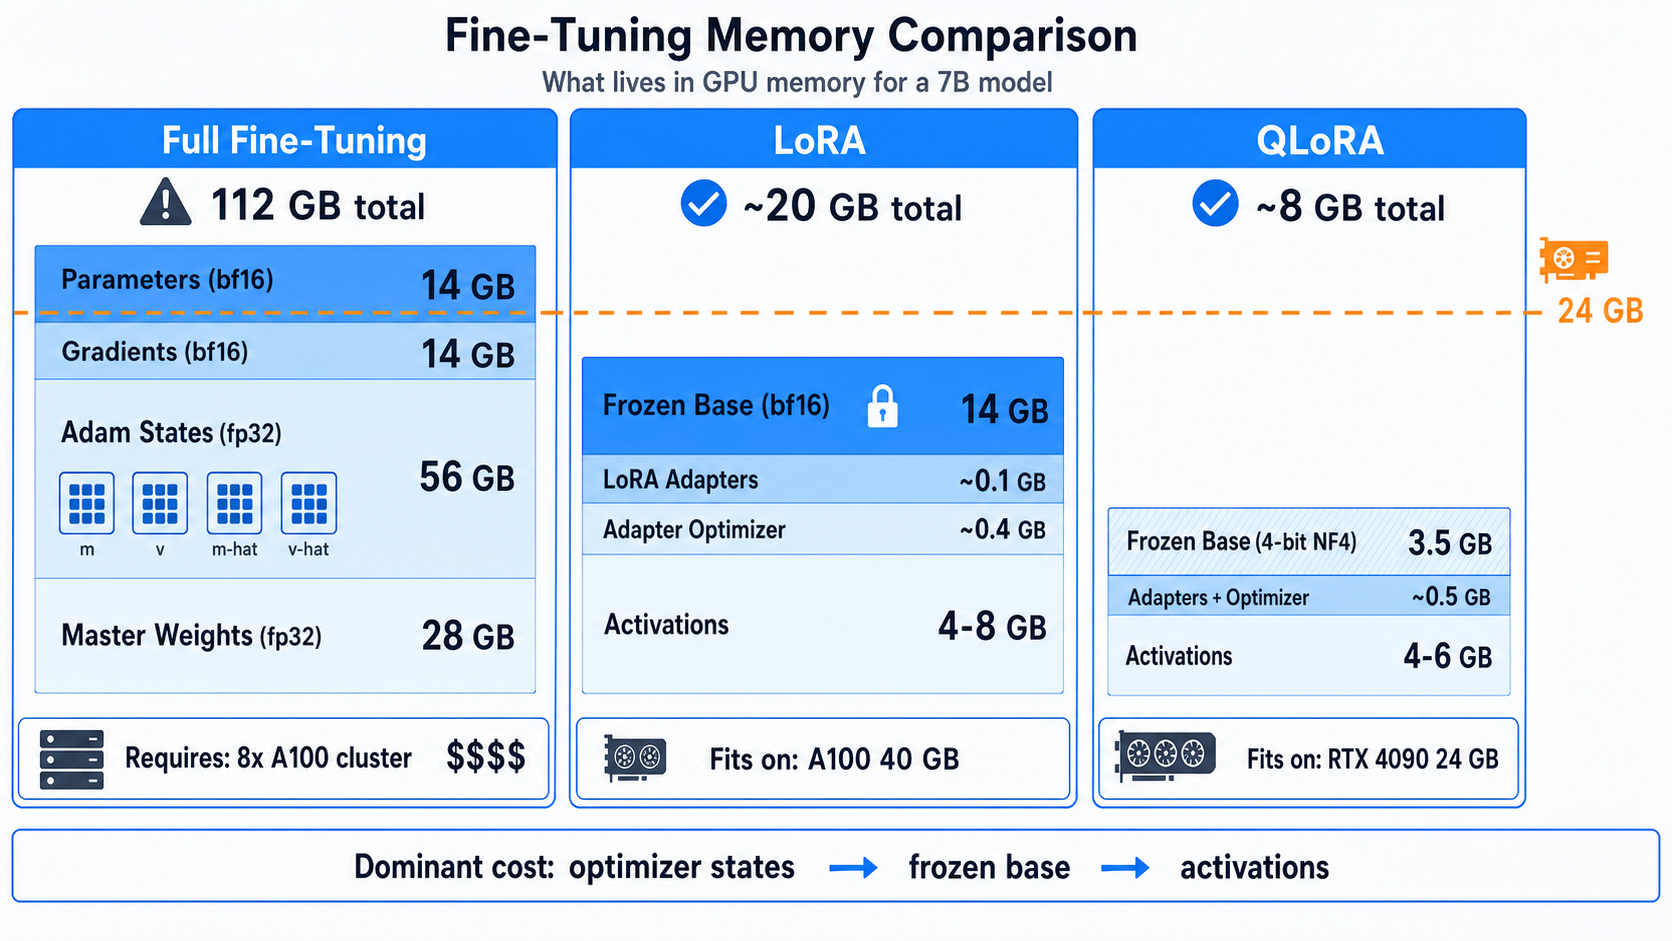
\includegraphics[width=0.92\textwidth]{figures/ch12/fig_memory_wall.png}
\caption{\textbf{The fine-tuning memory wall.} Peak GPU memory for full fine-tuning of a 7B model with Adam in mixed precision. Parameters and gradients account for 28\,GB; optimizer states and master weights add 84\,GB more. A single 24\,GB consumer GPU holds less than one-fifth of the requirement. LoRA and QLoRA progressively reduce the dominant terms.}
\label{fig:peft-memory-wall}
\end{figure}

\paragraph{Why not just use FSDP?} You can---and for 70B+ models, you must. But the whole point of post-training is that it should be accessible. The open-model ecosystem depends on researchers and small teams fine-tuning models on 1--4 GPUs. If fine-tuning requires the same cluster that pretraining used, the democratization promise of open weights is hollow.

\paragraph{Where the memory goes.} The 112\,GB subtotal above has a clear structure:

\begin{itemize}[nosep]
  \item \textbf{Parameters and gradients} (28\,GB): proportional to model size. Unavoidable if you update all parameters.
  \item \textbf{Optimizer states} (56\,GB): the dominant term. Adam stores two statistics per parameter. This is the \emph{largest single component}---more than 4$\times$ the parameters themselves.
  \item \textbf{Master weights} (28\,GB): the fp32 copy of weights needed for the optimizer update step in mixed-precision training.
\end{itemize}

The insight that unlocks PEFT: \emph{if you only update a small subset of parameters, you only need optimizer states for that subset}. Freeze 99\% of the model, train the remaining 1\%, and the 84\,GB of optimizer states plus master weights collapses to less than 1\,GB. The frozen parameters still need to be in memory for the forward pass, but they are stored only once, in the base precision (or quantized---see \S\ref{sec:qlora}).

\begin{quickrecap}
\textbf{Quick Recap.}
\begin{itemize}[nosep,leftmargin=1.5em]
  \item Full fine-tuning of a 7B model requires $\sim$120\,GB of GPU memory---$5\times$ what a consumer GPU provides.
  \item The dominant memory cost is optimizer states (Adam moments + master weights), not the parameters themselves.
  \item If you freeze most parameters and only train a small subset, optimizer states shrink proportionally---this is the PEFT idea.
\end{itemize}
\textit{Next: the specific reparameterization that makes this practical---LoRA.}
\end{quickrecap}


%======================================================================
% SECTION 12.2: LoRA Mathematics
%======================================================================
\section{LoRA: Train the Update, Not the Model}
\label{sec:lora-math}

Low-Rank Adaptation~\cite{hu2021lora} proposes a simple reparameterization. Instead of updating the full weight matrix $W \in \mathbb{R}^{d \times d}$, freeze $W$ and train a low-rank additive update:

\[
\boxed{h = \left(W + \frac{\alpha}{r}\, B A\right) x}
\]

where $B \in \mathbb{R}^{d \times r}$ and $A \in \mathbb{R}^{r \times d}$ with $r \ll d$. $B$ is initialized to zero (so the model starts from the pretrained behavior), and $A$ is initialized from a Gaussian. The frozen matrix $W$ is never updated; only $B$ and $A$ receive gradients.

\begin{figure}[t]
\centering
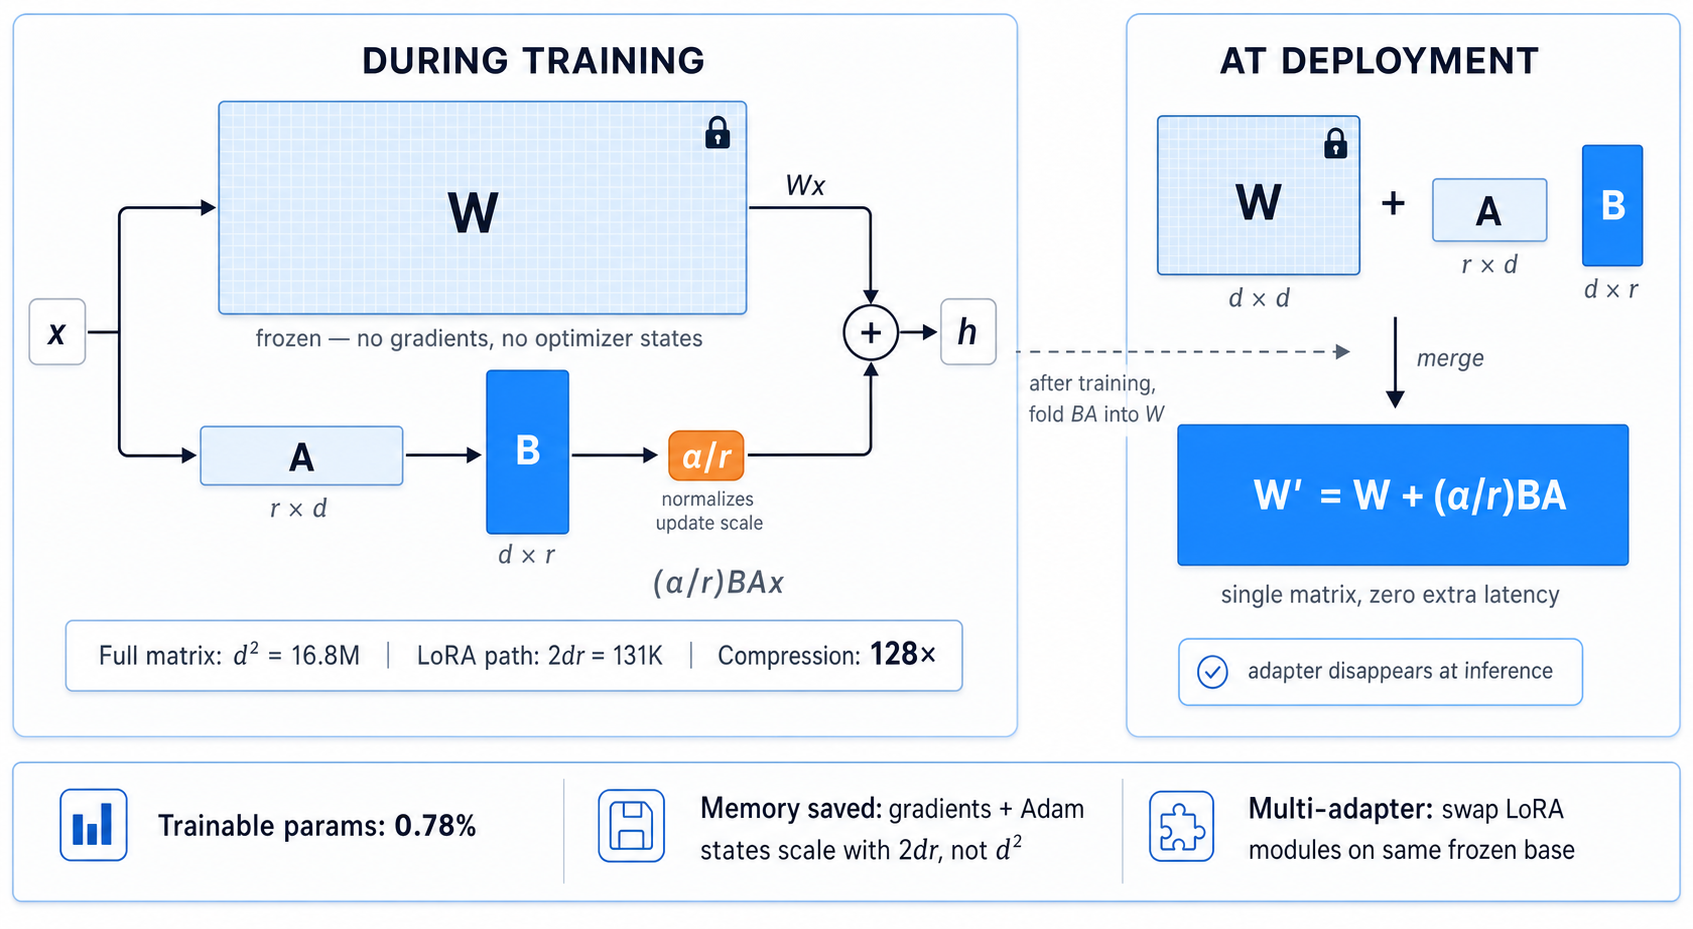
\includegraphics[width=0.9\textwidth]{figures/ch12/fig_lora_update.png}
\caption{\textbf{LoRA trains the update, not the base model.} The pretrained matrix $W$ remains frozen. A small low-rank path, $B A$, learns the task-specific update and is scaled by $\alpha/r$ before being added to the original projection. Because $r \ll d$, the trainable path is tiny relative to the frozen weight matrix.}
\label{fig:lora-update}
\end{figure}

\subsection{Parameter compression}

For a single $4096 \times 4096$ attention projection ($Q$, $K$, $V$, or $O$), the full weight matrix has $4096^2 = 16{,}777{,}216$ parameters. A rank-16 LoRA adapter has:
\[
2 \times 4096 \times 16 = 131{,}072 \quad \text{parameters}
\]
That is $0.78\%$ of the full matrix---a $128\times$ compression. But the real saving is not in parameter count. It is in \emph{optimizer states}: Adam needs two 32-bit statistics per trainable parameter. At $0.78\%$ trainable parameters, the optimizer state is $0.78\%$ of the full fine-tuning cost. The 56\,GB of Adam moments from \S\ref{sec:memory-wall-peft} collapses to $\sim$0.4\,GB.

\subsection{Which modules to adapt}

LoRA can be applied to any linear layer. In practice:

\begin{itemize}[nosep]
  \item \textbf{Attention projections only} ($Q$, $K$, $V$, $O$): the original LoRA paper's default. Captures most of the behavioral shift with minimal parameters.
  \item \textbf{All linear layers} (attention + MLP): more expressive but more parameters. Used when quality on the target task matters more than memory.
\end{itemize}

For Project~3 at 3B scale on a 24\,GB GPU, the recommended default is $Q$, $K$, $V$, $O$ projections with $r = 16$.

\subsection{\texorpdfstring{The $\alpha/r$ Scaling Factor}{The alpha/r Scaling Factor}}

The factor $\alpha/r$ in the LoRA forward pass is often treated as a minor implementation detail. It is not. Understanding it prevents a common pitfall when sweeping rank.

Without an explicit scaling convention, changing $r$ changes more than capacity. A larger rank gives the update more directions and changes the typical magnitude of gradients flowing through the LoRA path. If you increase $r$ from 8 to 32 and leave all other hyperparameters untouched, you are not just adding capacity; you are also changing the effective update scale.

The $\alpha/r$ factor normalizes this:
\[
\Delta W = \frac{\alpha}{r}\, BA
\]

The scaling factor separates two knobs that would otherwise be entangled: $r$ controls the capacity of the adapter, while $\alpha$ controls the update scale. This does not make rank sweeps perfectly invariant---optimization is still stochastic, and initialization matters---but it gives you a stable convention for comparing ranks.

\paragraph{Practical rule.} Set $\alpha = r$ for your first run. This gives $\alpha/r = 1$, a conservative starting point that is easy to reason about. When sweeping rank, decide explicitly whether you are keeping the scale ratio $\alpha/r$ fixed (so $\alpha$ grows with $r$) or keeping $\alpha$ fixed (so higher ranks get smaller per-rank scale). Do not compare ranks while accidentally changing both capacity and scale. Treat $\alpha$ as a learning-rate-like knob and report it whenever you report rank.

\begin{tcolorbox}[colback=orange!5, colframe=orange!60, title=\textbf{For Project~3: LoRA Configuration}]
\begin{itemize}[nosep]
  \item \textbf{Rank:} $r = 16$ (default; try $r = 32$ if quality plateaus).
  \item \textbf{Alpha:} $\alpha = 16$ (start with $\alpha = r$).
  \item \textbf{Target modules:} $Q$, $K$, $V$, $O$ projections (attention only).
  \item \textbf{LoRA dropout:} 0.05 (light regularization; optional).
  \item \textbf{Trainable parameters:} $\sim$0.5--1\% of total. At 3B, this is $\sim$15--30M parameters.
\end{itemize}
\end{tcolorbox}

\subsection{Merging at inference time}

After training, the LoRA update can be merged back into the base weights:
\[
W_{\text{merged}} = W + \frac{\alpha}{r}\, BA
\]
The result is a standard weight matrix with no architectural changes and \emph{zero inference overhead}. This is a key advantage over other PEFT methods: the adapter vanishes after training. You ship a single model, not a model plus an adapter module.

Alternatively, you can keep the adapter separate. This enables \emph{multi-adapter serving}: one base model in memory, with different LoRA adapters swapped in for different tasks or users. At 0.78\% of the base model's size, each adapter is small enough to store hundreds on disk and load on demand.

\begin{quickrecap}
\textbf{Quick Recap.}
\begin{itemize}[nosep,leftmargin=1.5em]
  \item LoRA freezes the pretrained weights $W$ and trains a low-rank update $\Delta W = \frac{\alpha}{r} BA$.
  \item Parameter compression is $\sim$$100\times$; optimizer state compression follows proportionally.
  \item The $\alpha/r$ factor separates adapter capacity from update scale; rank sweeps should report both $r$ and $\alpha$.
  \item After training, the adapter merges into $W$ with zero inference cost---or stays separate for multi-adapter serving.
\end{itemize}
\textit{Next: why this extreme compression works at all---the surprising low dimensionality of fine-tuning.}
\end{quickrecap}


%======================================================================
% SECTION 12.3: Why LoRA Works --- Intrinsic Dimension
%======================================================================
\section{Why LoRA Works: The Intrinsic Dimension of Fine-Tuning}
\label{sec:lora-why}

LoRA compresses a 16-million-parameter weight matrix into 131K trainable parameters and loses almost nothing. Why does a $128\times$ reduction in capacity produce a model of comparable quality? The answer predates LoRA by a year.

\paragraph{The Aghajanyan experiment.} Aghajanyan et al.\ (2021)~\cite{aghajanyan2021intrinsic} asked a simple question: what is the minimum number of free parameters needed to fine-tune a pretrained model to near-optimal performance? They did this by applying the Fastfood transform---a structured random projection---to restrict the update to a subspace of dimension $d_{\text{int}}$, then measuring how small $d_{\text{int}}$ could be before performance degraded.

The result was striking. For several standard NLP tasks, models with hundreds of millions of parameters achieved most of their full fine-tuning performance while the update was restricted to a subspace with only hundreds or thousands of dimensions. The exact number depends on task and model scale, but the qualitative lesson is stable: the useful update is dramatically smaller than the full parameter count.

\paragraph{What this means.} Fine-tuning does not explore the full parameter space. The gradient updates during fine-tuning behave as if they lie in a much smaller subspace---a low-dimensional manifold within the high-dimensional weight space. Pretraining has already found a good region; fine-tuning makes a small, directed adjustment within that region. The important comparison is not whether the intrinsic dimension is 200, 2{,}000, or 20{,}000. It is that all of those numbers are tiny compared with hundreds of millions or billions of parameters.

An analogy is useful. Full fine-tuning treats the pretrained model like a city whose every road can be rebuilt. LoRA treats it like a city whose road network already works: you add a small set of ramps, signs, and lane changes that redirect traffic toward the new destination. If the destination is nearby---instruction following, formatting, tone, safety style---small redirects are enough. If the destination is a different city---new facts, new language, new domain knowledge---small redirects may not suffice.

\begin{figure}[t]
\centering
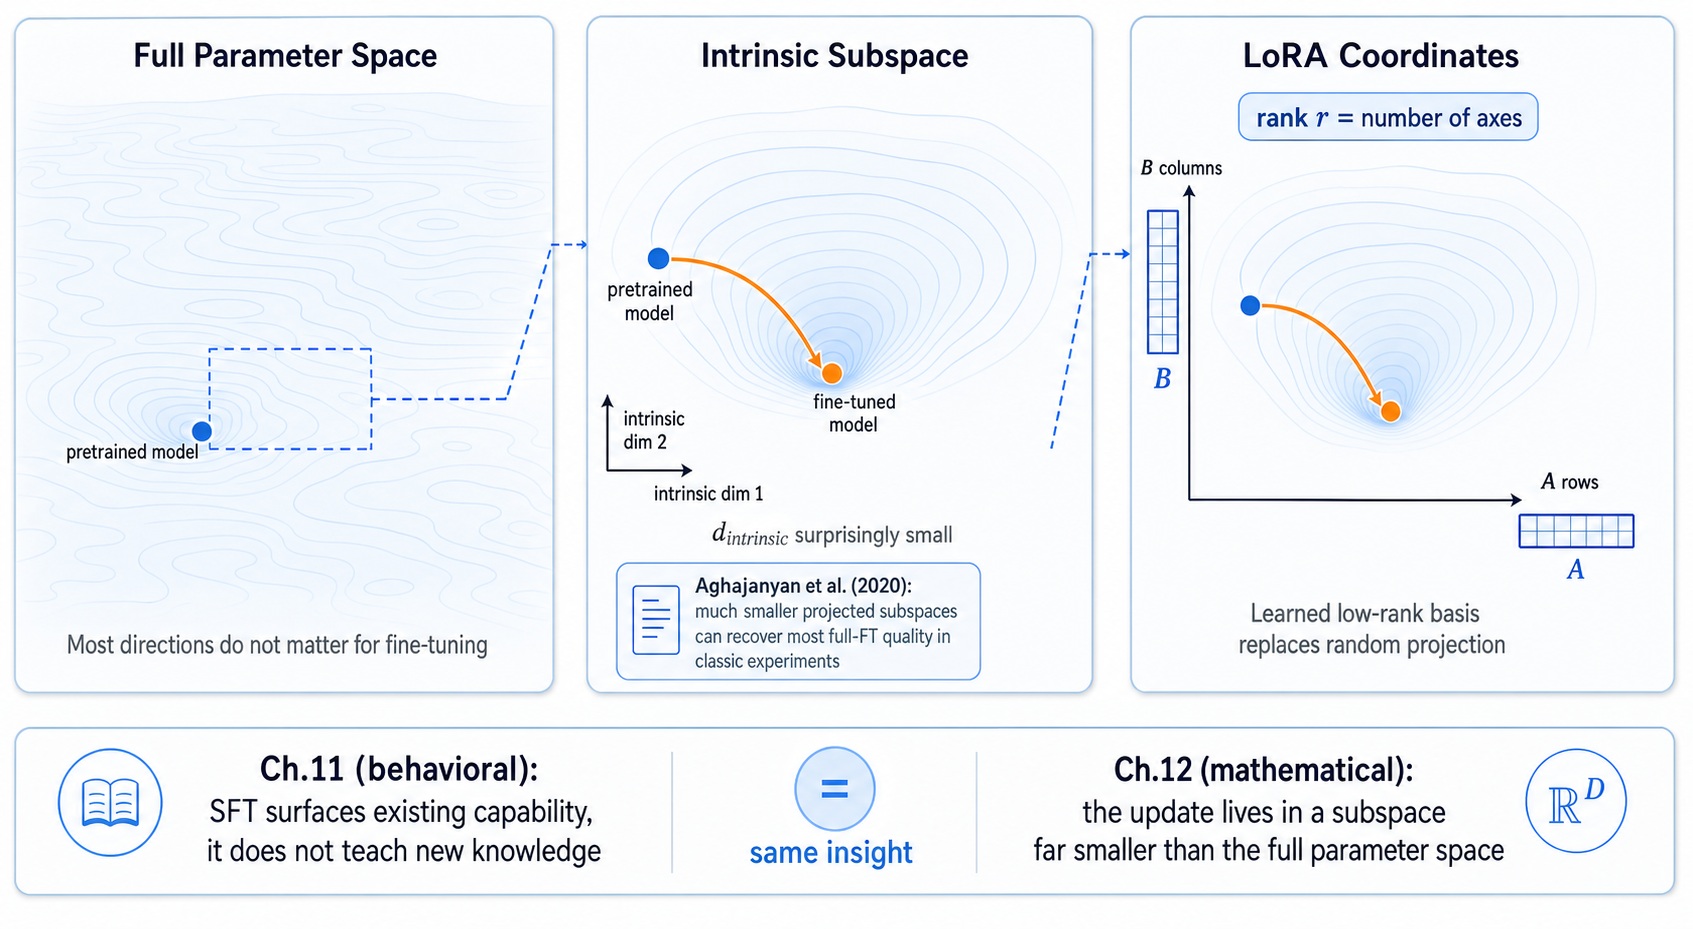
\includegraphics[width=0.92\textwidth]{figures/ch12/fig_intrinsic_dimension.png}
\caption{\textbf{The intrinsic dimension of fine-tuning.} A high-dimensional weight space (left) contains a low-dimensional subspace (right) in which the fine-tuning update lives. LoRA parameterizes this subspace explicitly as a low-rank matrix factorization, achieving comparable quality to full fine-tuning with $\sim$$100\times$ fewer trainable parameters.}
\label{fig:intrinsic-dimension}
\end{figure}

LoRA is the engineering realization of this insight. Instead of Aghajanyan's random projection (which is not practical for training), LoRA uses a \emph{learned} low-rank projection: the matrices $B$ and $A$ define a rank-$r$ subspace, and the optimizer learns the best update within that subspace. The rank $r$ is the intrinsic dimension budget that you allocate.

\begin{tcolorbox}[colback=gray!5, colframe=gray!50, title=\textbf{The LIMA--Aghajanyan Connection}]
Chapter~\ref{ch:instruction-tuning} argued \emph{behaviorally} that SFT does not teach new knowledge---it surfaces existing capability. The LIMA hypothesis (Zhou et al., 2023) crystallized this: 1{,}000 high-quality examples can redirect a 65B model because the capability was already there; SFT just needs to point the model in the right direction.

\medskip
The intrinsic dimensionality result is the \emph{mathematical} version of the same claim. If fine-tuning only needs a small subspace, the model is usually not learning a new language from scratch or rebuilding its world model; it is making a targeted correction to an already-capable system. Low intrinsic dimension and ``surfacing existing capability'' are two descriptions of the same phenomenon at different levels of abstraction.

\medskip
This connection explains both why PEFT works and where it does not. When the task requires \emph{redirecting} existing capability (instruction following, format compliance, style adaptation), the update is low-rank and LoRA matches full fine-tuning. When the task requires \emph{injecting new knowledge} (teaching the model facts it never saw during pretraining, adapting to a domain far from the pretraining distribution), the intrinsic dimension is higher, and LoRA may fall short. \S\ref{sec:peft-decision} returns to this distinction.
\end{tcolorbox}

\paragraph{Empirical evidence across scales.} The intrinsic dimensionality finding was originally demonstrated on encoder models. LoRA then showed that low-rank adaptation works for large decoder-only language models as well: small ranks such as $r=4$--$8$ were competitive with full fine-tuning on the tasks Hu et al.\ evaluated~\cite{hu2021lora}. Modern instruction-tuning practice usually uses somewhat larger ranks ($r=16$--$64$), not because the low-rank story failed, but because larger adapters are cheap and give useful margin. The practical lesson is conservative: the rank needed for high-quality adaptation grows far more slowly than the model's full parameter count.

\noindent\fbox{\parbox{\dimexpr\textwidth-2\fboxsep-2\fboxrule\relax}{%
\textbf{Pause and verify.}\quad A 3B model has $\sim$3 billion parameters. LoRA with $r = 16$ applied to all attention projections ($Q$, $K$, $V$, $O$) in a model with hidden dimension 3072 and 32 layers trains $4 \times 2 \times 3072 \times 16 \times 32 \approx 12{.}6$M parameters---about 0.4\% of the total.

\smallskip
\emph{Why does 0.4\% of the parameters capture the behavioral shift? Because the fine-tuning update lives in a low-dimensional subspace. LoRA allocates just enough rank to span that subspace. The other 99.6\% of parameters are already in the right place from pretraining.}
}}

\begin{quickrecap}
\textbf{Quick Recap.}
\begin{itemize}[nosep,leftmargin=1.5em]
  \item Fine-tuning has low intrinsic dimensionality: the useful update often lives in a subspace far smaller than the full parameter count.
  \item LoRA is the practical implementation of this insight: a learned low-rank projection instead of a random one.
  \item The LIMA ``surfacing'' thesis (behavioral) and intrinsic dimensionality (mathematical) describe the same phenomenon: pretraining puts the capability in place, fine-tuning makes a small redirect.
  \item Caveat: knowledge-injection tasks have higher intrinsic dimension, and LoRA may underperform full fine-tuning on these tasks.
\end{itemize}
\textit{Next: LoRA reduces optimizer memory. Can we also compress the frozen base model?}
\end{quickrecap}


%======================================================================
% SECTION 12.4: QLoRA
%======================================================================
\section{QLoRA: Compress the Frozen Base}
\label{sec:qlora}

LoRA eliminates most optimizer states. But the frozen base model is still in memory. A 7B model in bf16 occupies 14\,GB---more than half of a 24\,GB GPU, before any activations or LoRA parameters.

QLoRA~\cite{dettmers2023qlora} compresses the frozen base to 4-bit precision: 7B parameters at 4 bits fit in $\sim$3.5\,GB before quantization metadata. Combined with LoRA adapters (which remain in bf16), the model-state footprint drops dramatically. Peak training memory still depends on sequence length, batch size, activation checkpointing, and optimizer implementation, but the 7B case moves from ``impossible on 24\,GB'' to ``practical with careful settings,'' and a 3B model fits comfortably.

\subsection{NF4: Normal Float 4-bit}

Why not just use INT4? Standard 4-bit integer quantization divides the value range into 16 equally spaced bins. This is wasteful for neural network weights after blockwise normalization, which are approximately normally distributed: most values cluster near zero, and the tails are sparsely populated. Uniform bins over-represent the tails and under-represent the dense center.

NF4 (Normal Float 4-bit) solves this by defining the 16 representation values as the \emph{quantiles of the standard normal distribution}. Each bin contains an equal fraction of the probability mass under a Gaussian. Since normalized Transformer weight blocks are close to normal, NF4 bins match the actual data distribution better than uniform INT4, producing lower quantization error at the same bit width.

\begin{figure}[t]
\centering
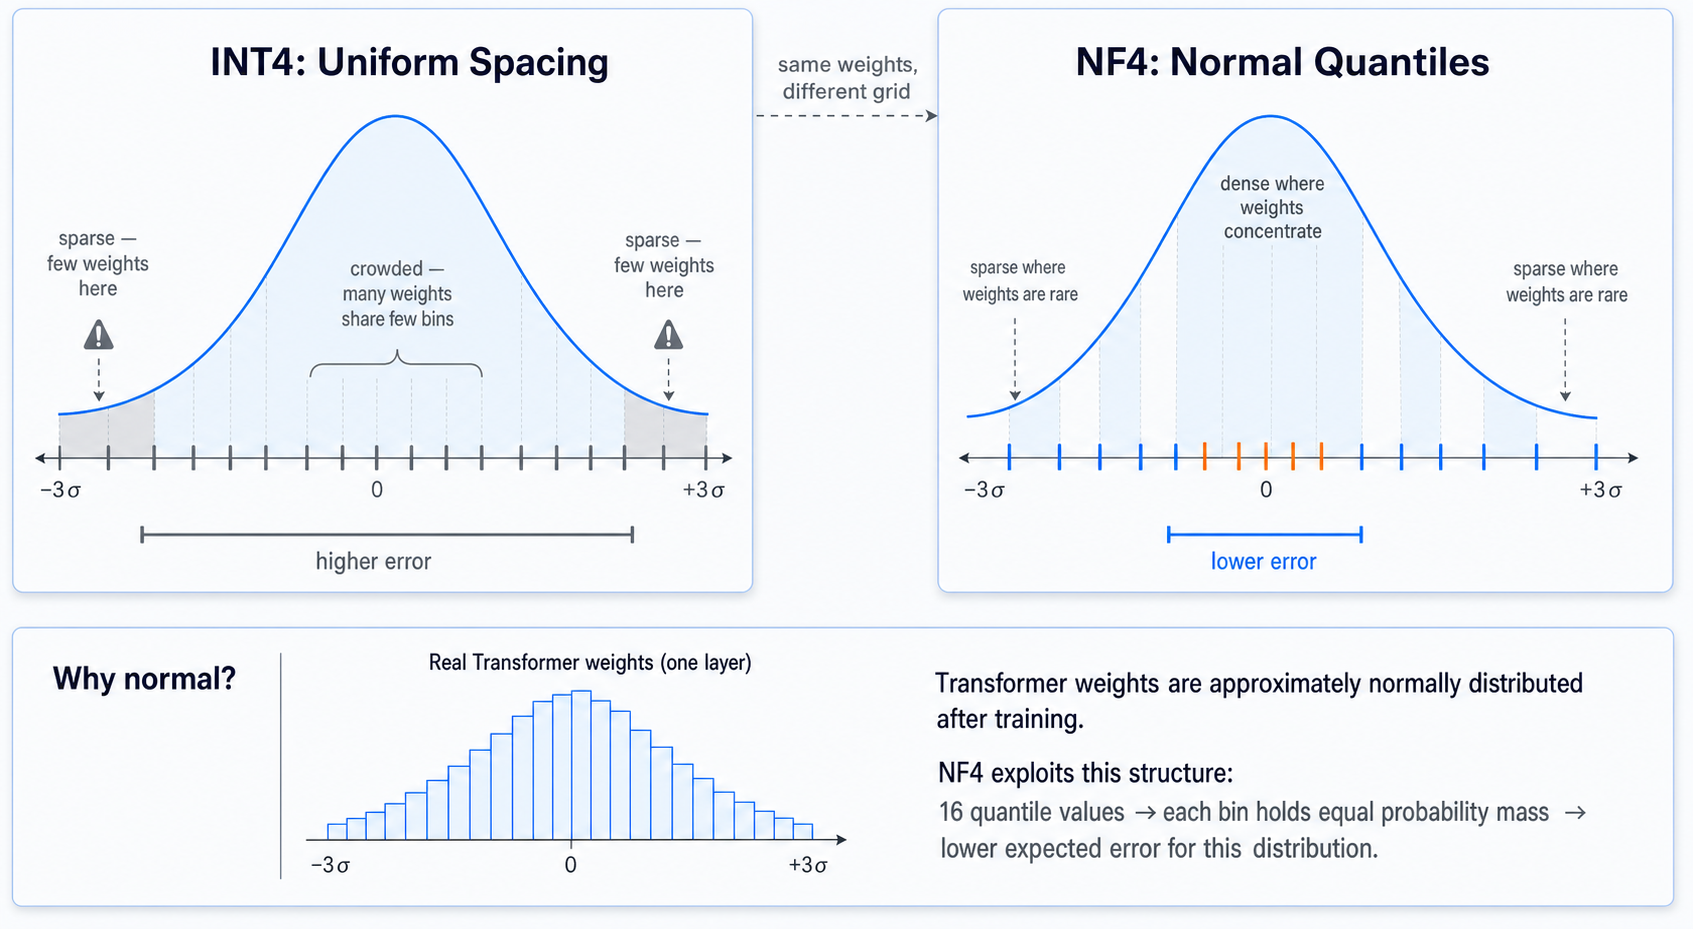
\includegraphics[width=0.85\textwidth]{figures/ch12/fig_nf4_quantization.png}
\caption{\textbf{NF4 vs.\ INT4 quantization.} INT4 divides the value range into 16 uniform bins (top), wasting precision on the sparse tails. NF4 places 16 representation values at the quantiles of the normal distribution (bottom), matching the empirical weight distribution. The result: lower quantization error per bit for normally distributed weights.}
\label{fig:nf4-quantization}
\end{figure}

The intuition is information-theoretic: if you know the distribution of the data, the optimal fixed-point quantizer places representation values to equalize the probability mass in each bin. For Gaussian data, that is the quantile grid. NF4 is approximately information-theoretically optimal for weights drawn from a normal distribution.

\subsection{Double quantization}

Quantization requires storing per-block scaling constants---one scalar for each block of weights. At 7B parameters, this overhead is small but not negligible. Double quantization quantizes these scaling constants themselves, saving about 0.37 bits per parameter in the QLoRA setup. The quality impact is small because the constants are metadata for a frozen base, not trainable weights.

\subsection{Paged optimizers}

When GPU memory is extremely tight, QLoRA uses NVIDIA's unified memory to let optimizer states spill from GPU to CPU RAM on demand. This is not fast---CPU memory bandwidth is $10\times$--$30\times$ slower than GPU HBM---but it prevents out-of-memory crashes during occasional memory spikes (e.g., long sequences in a batch). In practice, paging activates rarely and the throughput impact is small.

\subsection{When QLoRA matches full fine-tuning---and when it does not}

Dettmers et al.\ reported that QLoRA with NF4 produced instruction-tuned models competitive with 16-bit adapter tuning and strong open chat baselines. This result is consistent with the intrinsic dimensionality story: instruction tuning is a capability-surfacing task with low intrinsic dimension, so the small quality loss from 4-bit base quantization can often be absorbed by the LoRA adapter.

But this does not generalize to all tasks. When the fine-tuning objective requires the model to encode \emph{new information} not present in the pretrained weights---domain-specific knowledge injection, new language acquisition, or specialized factual recall---the 4-bit quantization of the base introduces a floor on representational fidelity. The frozen base cannot represent certain fine-grained weight distinctions that full-precision fine-tuning would preserve. In these settings, full fine-tuning or higher-precision LoRA (bf16 base + LoRA) may outperform QLoRA.

\begin{tcolorbox}[colback=blue!5, colframe=blue!60, title=\textbf{Does 4-bit Quantization Throw Away What Fine-Tuning Needs?}]
The right answer is task-dependent. For instruction tuning, the adapter mostly needs to redirect behavior already encoded in the base model, so a high-quality 4-bit representation is often enough. For knowledge injection, the exact numerical details of the base weights can matter more: the task is asking the model to store or retrieve information the base does not already organize well.

\medskip
This is why ``QLoRA matches full fine-tuning'' is too broad as a rule. A better rule is: QLoRA is a strong default for capability-surfacing post-training; use higher-precision LoRA or full fine-tuning when the objective is to change the model's knowledge, not just its behavior.
\end{tcolorbox}

\begin{tcolorbox}[colback=orange!5, colframe=orange!60, title=\textbf{For Project~3: QLoRA Setup}]
\begin{itemize}[nosep]
  \item \textbf{Base precision:} NF4 (4-bit). At 3B parameters, the base model occupies $\sim$1.5\,GB.
  \item \textbf{LoRA precision:} bf16. Adapters are small ($\sim$30\,MB at $r = 16$).
  \item \textbf{Total estimated memory:} $\sim$4--8\,GB (depending on batch size and sequence length). Fits a 24\,GB GPU with room for batch size 4--8 at 2K tokens.
  \item \textbf{Task type:} Instruction tuning (capability surfacing). QLoRA is the recommended default; compare against bf16 LoRA if quality is unexpectedly brittle.
\end{itemize}
\end{tcolorbox}

\begin{quickrecap}
\textbf{Quick Recap.}
\begin{itemize}[nosep,leftmargin=1.5em]
  \item QLoRA compresses the frozen base model to 4-bit (NF4), reducing its memory footprint by $\sim$$4\times$.
  \item NF4 places representation values at normal distribution quantiles, matching the empirical weight distribution.
  \item Double quantization and paged optimizers squeeze out additional savings.
  \item QLoRA matches full fine-tuning on capability-surfacing tasks (instruction tuning) but may fall short on knowledge-injection tasks where the base representation matters more.
\end{itemize}
\textit{Next: LoRA is not the only PEFT method. What else exists, and why does LoRA dominate?}
\end{quickrecap}


%======================================================================
% SECTION 12.5: Other PEFT Methods
%======================================================================
\section{Beyond LoRA: The PEFT Landscape}
\label{sec:other-peft}

LoRA is the default in this course, but it was not the first attempt to make fine-tuning cheap. Before LoRA, researchers tried several ways to avoid updating the full model: insert small modules, prepend learned context, rescale internal activations, or train only a few selected parameters. This section is not a catalog for its own sake. It asks why these alternatives were plausible, and why LoRA became the practical default for the post-training workloads in Part~III.

\subsection{Adapter layers}

The earliest PEFT idea was to leave the Transformer intact and add small trainable modules around it. If the base model is a large frozen machine, adapters are small control boards attached between its parts.

Houlsby et al.\ (2019)~\cite{houlsby2019adapters} introduced small bottleneck modules inserted between Transformer layers: a down-projection ($d \to r$), a nonlinearity, and an up-projection ($r \to d$), plus a residual connection. The pretrained weights are frozen; only the adapter modules are trained.

Adapters work, but they introduce \emph{inference overhead}: the adapter modules remain in the forward pass at serving time. LoRA's update merges into $W$ and vanishes; adapters do not. For latency-sensitive deployments, this is a meaningful disadvantage.

\subsection{Prefix tuning}

Another route is to avoid changing weights at all. Instead of modifying the model, prefix tuning learns a continuous prompt that steers the model from the input side.

Li \& Liang (2021)~\cite{li2021prefix} prepend learnable ``virtual tokens'' to the key and value matrices at every layer. These tokens are not real text---they are continuous embeddings optimized during training. The pretrained weights are entirely frozen; only the prefix embeddings are trained.

Prefix tuning is parameter-efficient but has two limitations. First, the learnable prefixes consume context-window budget: a 20-token prefix reduces the available context by 20 tokens at every layer. Second, like adapters, the prefixes must be present at inference time---they do not merge away.

\subsection{\texorpdfstring{IA$^3$}{IA3}}

If adapters add modules and prefixes add context, IA$^3$ asks for an even smaller intervention: rescale the activations already flowing through the network.

IA$^3$ (Liu et al., 2022) multiplies activations by learned scaling vectors---element-wise rescaling of keys, values, and feedforward outputs. It is extremely parameter-efficient (far fewer parameters than LoRA) but limited in expressivity: scaling cannot represent the transformations that a low-rank additive update can.

\subsection{DoRA}

Modern variants mostly refine LoRA rather than replace it. DoRA is the most important example: it keeps the low-rank adaptation idea but changes what part of the weight update receives that adaptation.

DoRA (Liu et al., 2024)~\cite{liu2024dora} decomposes the weight matrix into magnitude and direction, then applies LoRA only to the direction component. This separation allows the model to independently adjust ``how much'' (magnitude) and ``which way'' (direction). Empirically, DoRA sometimes outperforms LoRA on fine-grained tasks, but it is not yet the community default and introduces modest additional complexity.

\subsection{Why LoRA dominates}

The PEFT landscape has converged on LoRA and QLoRA as the default for five engineering reasons:

\begin{enumerate}[nosep]
  \item \textbf{Merge-away inference}: the trained adapter merges into $W$, producing a standard model with zero serving overhead. Adapters and prefix tuning cannot do this.
  \item \textbf{Multi-adapter composability}: one base model serves multiple tasks by swapping LoRA adapters. This enables multi-tenant serving at minimal cost.
  \item \textbf{Quality}: on instruction tuning and preference alignment, LoRA matches full fine-tuning quality in most evaluations.
  \item \textbf{QLoRA stack}: 4-bit base + LoRA is a natural combination. No other PEFT method has a comparably mature quantization extension.
  \item \textbf{Implementation maturity}: training code, checkpoint formats, adapter merging, and serving patterns are most mature for LoRA. Adapter layers and prefix tuning remain useful ideas, but they are less often the default path for modern instruction tuning and preference tuning.
\end{enumerate}

This is not a claim that LoRA is theoretically superior. Adapter layers have a cleaner theoretical story (they do not assume low-rank structure), and prefix tuning can be advantageous in certain multi-tenant caching setups. But for the scenarios this course covers---SFT, DPO, and RL fine-tuning of 1B--70B models---LoRA is the right default.

\begin{quickrecap}
\textbf{Quick Recap.}
\begin{itemize}[nosep,leftmargin=1.5em]
  \item Adapter layers insert bottleneck modules but add inference latency.
  \item Prefix tuning learns virtual tokens but consumes context budget and does not merge away.
  \item IA$^3$ and DoRA are interesting variants with specific trade-offs.
  \item LoRA dominates in practice because of merge-away inference, multi-adapter composability, quality parity, the QLoRA stack, and mature implementation patterns.
\end{itemize}
\textit{Next: a decision framework for choosing between full fine-tuning, LoRA, and QLoRA.}
\end{quickrecap}


%======================================================================
% SECTION 12.6: Decision Tree
%======================================================================
\section{Choosing Full Fine-Tuning, LoRA, or QLoRA}
\label{sec:peft-decision}

The reader who has followed this chapter so far knows what LoRA and QLoRA are, why they work, and what their limitations are. This section converts that understanding into a decision procedure.

\begin{figure}[t]
\centering
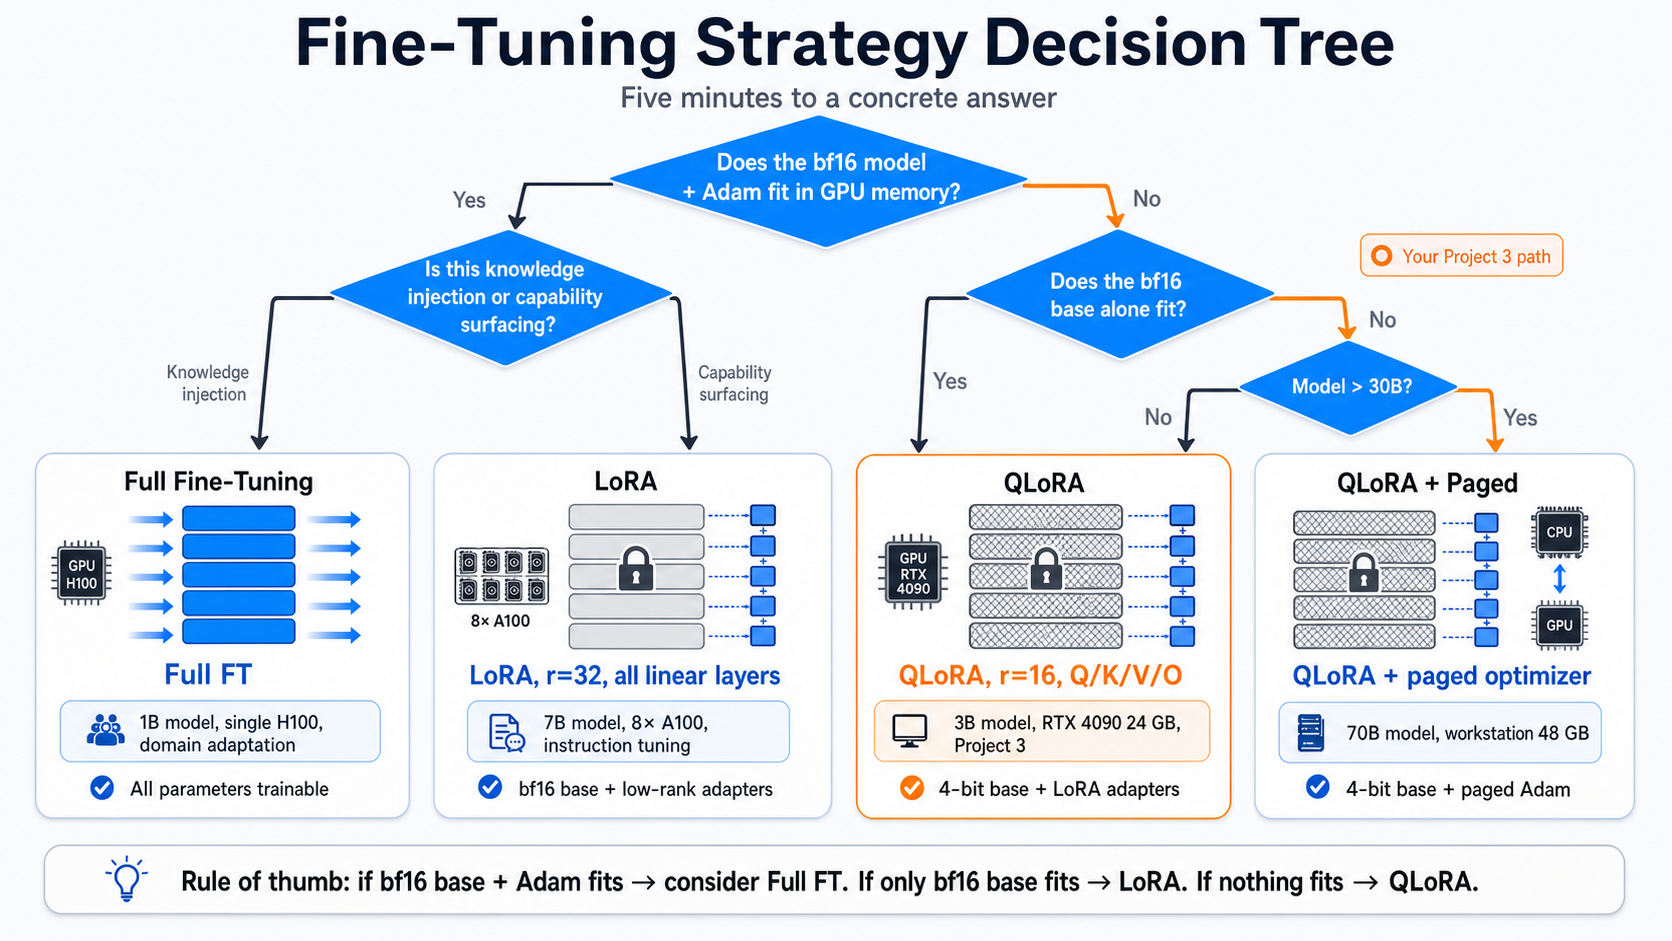
\includegraphics[width=0.92\textwidth]{figures/ch12/fig_decision_tree.png}
\caption{\textbf{Full FT vs.\ LoRA vs.\ QLoRA: a decision tree.} Four inputs---model size, available GPU memory, deployment requirements, and task type---determine the recommended fine-tuning strategy. The four worked examples below trace paths through this tree.}
\label{fig:decision-tree}
\end{figure}

\paragraph{Four inputs.}

\begin{enumerate}[nosep]
  \item \textbf{Model size}: how many parameters does the base model have?
  \item \textbf{Available GPU memory}: single 24\,GB consumer GPU, single 80\,GB A100, or multi-GPU?
  \item \textbf{Deployment requirements}: does the adapter need to merge for zero-overhead serving? Will you serve multiple adapters from one base?
  \item \textbf{Task type}: is the task capability-surfacing (instruction following, format compliance, style) or knowledge-injection (new domain facts, new language)?
\end{enumerate}

\paragraph{Decision rules.}

\begin{itemize}[nosep]
  \item If full fine-tuning fits in memory (model size $\leq$ 1--3B, or multi-GPU available) \emph{and} the task requires knowledge injection: \textbf{use full fine-tuning}.
  \item If full fine-tuning does not fit but the base model at bf16 fits: \textbf{use LoRA}.
  \item If even the bf16 base does not fit comfortably on a single card: \textbf{use QLoRA}.
  \item If the task is capability-surfacing and both LoRA and QLoRA fit: \textbf{prefer QLoRA when memory or throughput is the constraint}; prefer bf16 LoRA when you want to remove quantization as an experimental variable.
\end{itemize}

\paragraph{Four worked examples.}

\begin{center}
\begin{tabularx}{\textwidth}{@{}p{3cm}p{2.5cm}p{2.5cm}p{2.5cm}X@{}}
\toprule
\textbf{Scenario} & \textbf{Model} & \textbf{GPU} & \textbf{Task} & \textbf{Recommendation} \\
\midrule
Project~3 & 3B & 1$\times$ 24\,GB & Instruction tuning & \textbf{QLoRA}, $r = 16$, target $Q/K/V/O$ \\
Academic research & 7B & 8$\times$ A100 & Instruction tuning & \textbf{LoRA}, $r = 32$, all linear layers \\
Single workstation & 70B & 1$\times$ 80\,GB & Instruction tuning & \textbf{QLoRA} + paged optimizer \\
Small model & 1B & 1$\times$ H100 & Domain adaptation & \textbf{Full FT}---memory is not a constraint \\
\bottomrule
\end{tabularx}
\end{center}

\noindent\fbox{\parbox{\dimexpr\textwidth-2\fboxsep-2\fboxrule\relax}{%
\textbf{Pause and verify.}\quad Your team has a 13B base model, a single 48\,GB A6000, and wants to instruction-tune for code generation (a capability the base model already has from pretraining). Which method do you choose?

\smallskip
\emph{The 13B base in bf16 is $\sim$26\,GB---full FT is far beyond the card, and bf16 LoRA may fit only with careful activation checkpointing and small batches. QLoRA with an NF4 base ($\sim$6.5\,GB before metadata) leaves much more room. The task (code generation instruction-following) is capability-surfacing, so QLoRA is the safer first run. Answer: QLoRA, $r = 16$--$32$, target all attention projections; compare to bf16 LoRA later if you have memory headroom.}
}}

\begin{quickrecap}
\textbf{Quick Recap.}
\begin{itemize}[nosep,leftmargin=1.5em]
  \item Four inputs determine the choice: model size, GPU memory, deployment needs, and task type.
  \item Full FT when it fits and the task is knowledge-injection. LoRA when the bf16 base fits and you want to avoid quantization. QLoRA when the bf16 base is too large or when memory headroom matters more than removing every quantization variable.
  \item Project~3: QLoRA, $r = 16$, $Q/K/V/O$, on a single 24\,GB GPU.
\end{itemize}
\textit{Next: PEFT is not just for SFT. It is infrastructure for the rest of Part~III.}
\end{quickrecap}


%======================================================================
% SECTION 12.7: PEFT Across the Post-Training Pipeline
%======================================================================
\section{PEFT Across the Post-Training Pipeline}
\label{sec:peft-pipeline}

So far, this chapter has discussed PEFT in the context of SFT (Chapter~\ref{ch:instruction-tuning}). But every subsequent post-training method in Part~III also benefits from---and in many cases, \emph{requires}---PEFT. The reason is simple: post-training methods beyond SFT need multiple models in memory simultaneously.

\subsection{DPO with LoRA (Chapter~\ref{ch:preference-learning})}

DPO requires two sets of logits during training: the \textbf{policy model} (being updated) and the \textbf{reference model} (frozen, used to compute the KL constraint). Without PEFT, this often means two full model copies in memory---at 7B, $2 \times 14 = 28$\,GB in bf16 just for weights, before any gradients or optimizer states.

With LoRA, the memory layout is far more efficient:

\begin{itemize}[nosep]
  \item The \textbf{reference model} is the base weights $W$ (frozen, stored once in NF4: $\sim$3.5\,GB for 7B).
  \item The \textbf{policy model} is the same base weights $W$ plus a LoRA adapter $\Delta W = \frac{\alpha}{r} BA$ (adapter: $\sim$0.1\,GB).
  \item The two models \emph{share the base}: no second copy needed.
\end{itemize}

The reference logits are computed with the base weights alone; the policy logits use the base plus adapter. In an efficient implementation, both forward passes share the same frozen base, and only the adapter is trainable. PEFT does not make DPO free---activation memory, chosen/rejected pairs, and reference forward passes still matter---but it changes the dominant term: the second policy is no longer a second trainable copy of the model.

\subsection{PPO/RLHF with LoRA (Chapter~\ref{ch:rlhf})}

PPO requires four model roles: the \textbf{policy}, the \textbf{reference policy}, the \textbf{value model} (critic), and the \textbf{reward model}. In the naive layout, four full copies of a 7B model would require $\sim$56\,GB of weights alone---before gradients, optimizer states, or activations.

With PEFT, the policy and reference can share a base (as in DPO). The value model and reward model may be implemented as separate heads or separate adapters on a shared architecture, or as smaller auxiliary models; the exact layout is implementation-dependent. The savings are dramatic, but 7B PPO on a single 24\,GB GPU remains tight---rollout batches, activation memory, and multiple forward passes make it feasible only with aggressive checkpointing and small batches.

\subsection{GRPO/Reasoning RL with LoRA (Chapter~\ref{ch:reasoning-rl})}

GRPO eliminates the value model entirely (Chapter~\ref{ch:reasoning-rl} explains why). This removes one of PPO's memory bottlenecks. The remaining roles---policy, reference, and reward or verifier---are easier to arrange around a shared quantized base plus adapters. The lighter memory profile is one reason open-source reasoning-RL experiments often use LoRA or QLoRA rather than full fine-tuning.

\paragraph{The infrastructure argument.} This section is the reason Chapter~\ref{ch:peft} is placed before Chapter~\ref{ch:preference-learning} in the book, not after. PEFT is not a one-chapter optimization trick that you can skip. It is \emph{load-bearing infrastructure} for the rest of Part~III. When Chapter~\ref{ch:preference-learning} describes DPO training, it will assume you understand why the reference model does not require a second memory budget. When Chapter~\ref{ch:rlhf} describes PPO, it will assume you understand the shared-base layout. This chapter gave you that understanding.

\begin{quickrecap}
\textbf{Quick Recap.}
\begin{itemize}[nosep,leftmargin=1.5em]
  \item DPO needs policy and reference logits. With LoRA, an efficient implementation can share the base and train only the adapter.
  \item PPO needs multiple model roles. PEFT reduces the dominant weight and optimizer-state terms, though activations and rollout batches still make PPO memory-hungry.
  \item GRPO drops the value model, making LoRA-based reasoning RL more accessible than PPO-style RLHF.
  \item PEFT is infrastructure for Chapters~\ref{ch:preference-learning}--\ref{ch:reasoning-rl}, not just a cost optimization for SFT.
\end{itemize}
\end{quickrecap}


%----------------------------------------------------------------------
% KEY TAKEAWAYS
%----------------------------------------------------------------------
\begin{takeaways}
\textbf{Key Takeaways}
\begin{itemize}[nosep]
  \item Full fine-tuning of large models is bottlenecked by optimizer state memory, not parameter count. A 7B model requires $\sim$120\,GB---$5\times$ a consumer GPU.
  \item LoRA trains a low-rank additive update $\Delta W = \frac{\alpha}{r} BA$ while freezing the pretrained weights, reducing trainable parameters by $\sim$$100\times$ and optimizer states proportionally.
  \item This works because fine-tuning has low intrinsic dimensionality: the useful update lives in a subspace far smaller than the full weight space. This is the mathematical counterpart of the LIMA ``surfacing'' thesis.
  \item QLoRA compresses the frozen base to 4-bit (NF4), cutting the base model's memory by $\sim$$4\times$ and making 7B fine-tuning practical on a 24\,GB GPU with careful settings.
  \item LoRA dominates the PEFT landscape because of merge-away inference, multi-adapter composability, quality parity on capability-surfacing tasks, the QLoRA extension, and mature implementation patterns.
  \item PEFT is infrastructure for all post-training methods: DPO, PPO, and GRPO all require multiple model roles, and PEFT makes those roles feasible on accessible hardware.
\end{itemize}
\end{takeaways}


%----------------------------------------------------------------------
\section*{Summary}

\paragraph{What this chapter established.} Parameter-efficient fine-tuning transforms post-training from a cluster-scale operation into something a single researcher can do on a consumer GPU. The key idea is simple: if you only update 1\% of the model's parameters, you only pay 1\% of the optimizer memory. LoRA implements this by training a low-rank additive update while freezing the pretrained weights; QLoRA extends it by compressing the frozen base to 4-bit precision.

\paragraph{The low-rank insight.} The most important idea in this chapter is not the memory savings---those are the engineering consequence. The important idea is the \emph{reason} the savings are possible: fine-tuning operates in a low-dimensional subspace of the full parameter space. Aghajanyan et al.\ showed this empirically; LoRA exploits it practically. This is the same insight that Chapter~\ref{ch:instruction-tuning}'s LIMA discussion reached from the behavioral side: pretraining puts the capability in place, and fine-tuning makes a small redirect. The data matters more than the number of parameters you update.

\paragraph{One sentence.} Fine-tuning does not need the full parameter space---so it should not require the full hardware stack.

\paragraph{What comes next.} Chapter~\ref{ch:preference-learning} moves beyond imitation learning. Instead of demonstrating the desired behavior, you provide \emph{pairwise preferences}---which response is better---and the model learns to produce preferred outputs. The DPO loss will look unfamiliar, but the training infrastructure (LoRA, shared base, reference model) is exactly what this chapter prepared you for.


%----------------------------------------------------------------------
\section*{Key Equations at a Glance}

\begin{center}
\begin{tabularx}{\textwidth}{@{}p{5cm}X@{}}
\toprule
\textbf{Quantity} & \textbf{Expression} \\
\midrule
LoRA forward pass & $h = \left(W + \frac{\alpha}{r}\, BA\right) x$ \\[4pt]
LoRA parameter count (per projection) & $2 \times d \times r$ \quad vs.\ $d^2$ for full \\[4pt]
LoRA compression ratio & $\frac{d}{2r}$ \quad (e.g., $d = 4096$, $r = 16$ $\Rightarrow$ $128\times$) \\[4pt]
QLoRA memory (base) & $\frac{\text{params} \times 4\,\text{bits}}{8} \approx \frac{\text{params}}{2}$ bytes \\[4pt]
Full FT peak memory (approx.) & $\underbrace{4P}_\text{params+grads} + \underbrace{12P}_\text{Adam+master}$ bytes (mixed precision) \\
\bottomrule
\end{tabularx}
\end{center}


%----------------------------------------------------------------------
\section*{Key Readings}

\begin{enumerate}[nosep]
  \item \textbf{Hu et al., 2021.} ``LoRA: Low-Rank Adaptation of Large Language Models.'' The foundational paper. Read for the reparameterization, the GPT-3 experiments, and the comparison to full fine-tuning.
  \item \textbf{Aghajanyan et al., 2021.} ``Intrinsic Dimensionality Explains the Effectiveness of Language Model Fine-Tuning.'' The theoretical motivation for why low-rank updates work. Essential for understanding \emph{why}, not just \emph{how}.
  \item \textbf{Dettmers et al., 2023.} ``QLoRA: Efficient Finetuning of Quantized LLMs.'' NF4 quantization + LoRA. Changed the accessibility of fine-tuning for the open-source community.
  \item \textbf{Houlsby et al., 2019.} ``Parameter-Efficient Transfer Learning for NLP.'' The original adapter paper. Read for historical context and to understand the design choices LoRA improved upon.
  \item \textbf{Li \& Liang, 2021.} ``Prefix-Tuning: Optimizing Continuous Prompts for Generation.'' An alternative PEFT paradigm. Useful for understanding the design space LoRA sits within.
\end{enumerate}

\flushbottom
